%versi 3 (22-07-2020)
\chapter{Analisis}
\label{chap:analisis}
Pada bab ini akan dijelaskan mengenai proses pengumpulan data citra satelit yang berada di Hadoop LAB Unpar, pengkonversian data \textit{text} menjadi gambar, dan bagaimana cara penggabungan gambar. Juga akan menjelaskan tetang analisis kebutuhan dalam perancangan perangkat lunak. 

\section{Proses Pembentukan Gambar}
Pada Gambar \ref{fig:ciumbuleuit} merupakan hasil dari penggabungan gambar per \textit{tile}. Langkah-langkah dalam proses pengambilan data berupa gambar citra satelit dari kecamatan atau kelurahan di Kota Bandung. 
\begin{figure}[H]
	\centering
	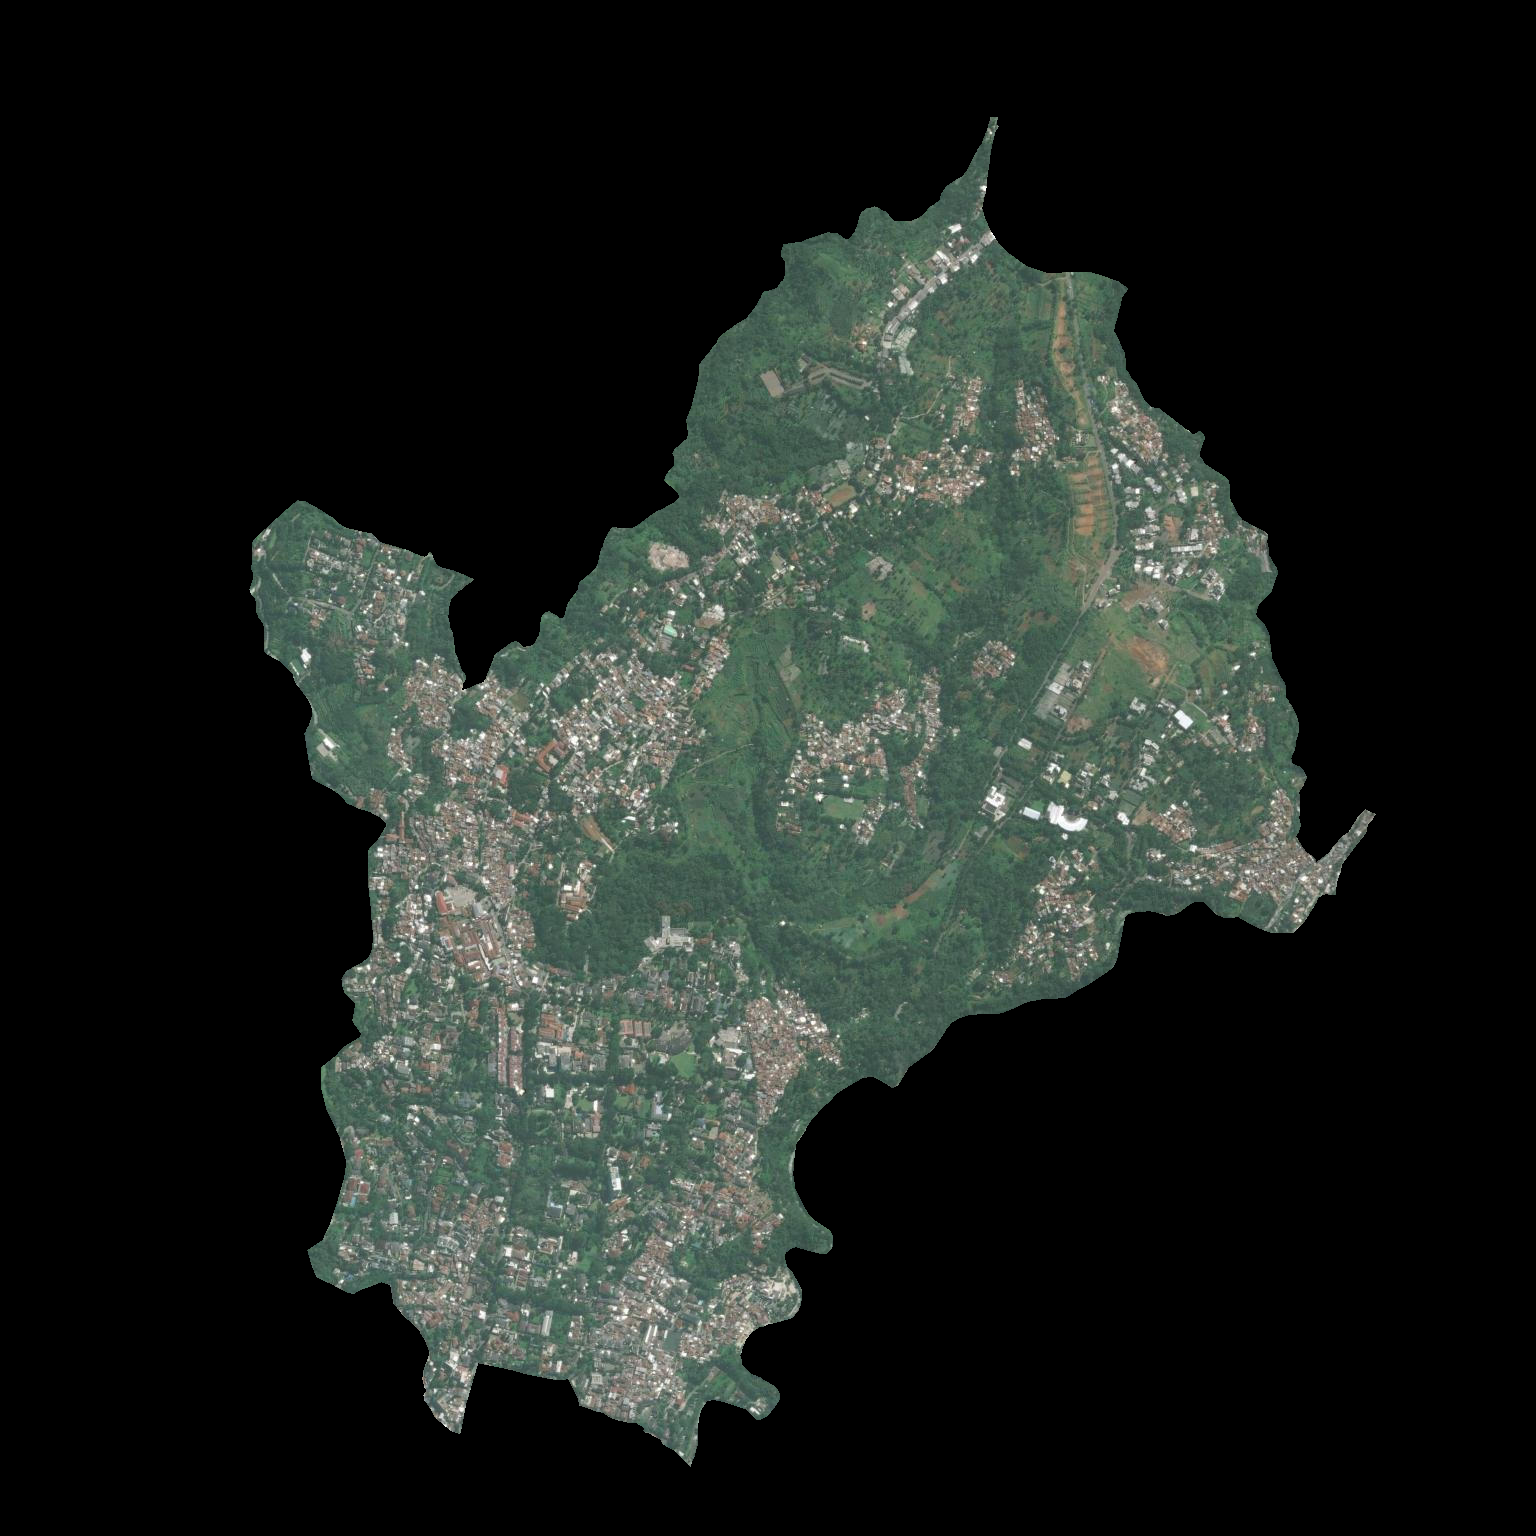
\includegraphics[width=0.5\textwidth]{Gambar/Ciumbuleuit.png}
	\caption{Gambar seluruh tile dari kelurahan Ciumbuleuit}
	\label{fig:ciumbuleuit}
\end{figure} 

Pertama-tama data yang diambil dari sistem Hadoop yang disimpan pada Hadoop Laboratoium Unpar. Kemudian data yang telah diambil berupa file ".txt" yang setiap baris dari file tersebut merupakan sebuah file gambar berupa \textit{tile} seperti pada gambar(\ref{fig:tileCiumbuleuit}). Kumpulan gambar per \textit{tile} akan digabungkan dengan menggunakan \textit{script}. Penggabungan gambar setiap \textit{tile} akan menghasilkan sebuah gambar dari kecamatan/kelurahan seperti pada gambar \ref{fig:ciumbuleuit}.

\begin{figure}[htp]
	\centering
	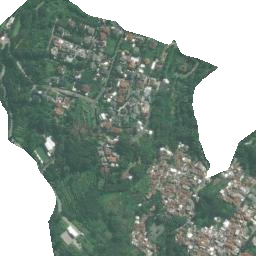
\includegraphics[scale=0.4]{Ciumbuleuit21.png}
	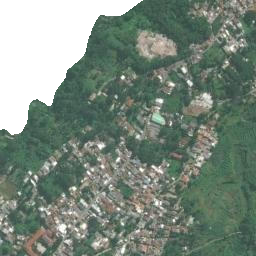
\includegraphics[scale=0.4]{Ciumbuleuit22.png}
	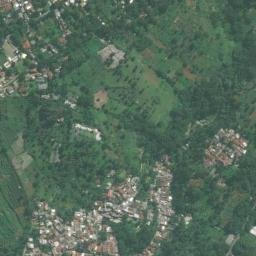
\includegraphics[scale=0.4]{Ciumbuleuit23.png}
	\caption{Contoh gambar kelurahan Ciumbuleuit setiap \textit{tile}}
	\label{fig:tileCiumbuleuit}
\end{figure}

\subsection{Mengunduh File Text}


\subsection{Mengkonversi Baris Menjadi Gambar .png}
\subsection{Menggabungkan Gambar}

\section{Analisis Perangkat Lunak}
Proses analisis perangkat lunak merupakan kebutuhan yang memerlukan peranan seorang pengguna untuk menjalankan sebuah perangkat lunak yang akan dikembankan. Sehingga segala proses sistem dijalankan oleh aktor yang terlibat. Dalam sistem ini hanya memiliki aktor sebagai \textit{user}. Seorang pemangku kepentingan atau pembuat keputusan memegang peranan sebagai \textit{user} itu sendiri. Dalam menggambarkan peranan pengguna terhadap interaksinya dengan sistem, maka dapat dilihat pada diagram \textit{use case} yang terdapat pada Gambar~\ref{fig:useCaseUser} berikut.

\begin{figure}[H]
	\centering
	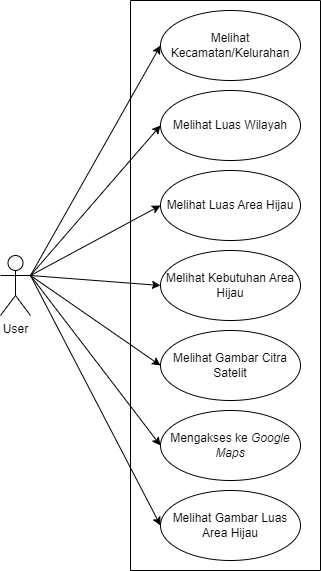
\includegraphics[scale=0.5]{Gambar/UseCaseUser.png}
	\caption[Diagram \textit{Use Case} \textit{User}]{Diagram \textit{Use Case} \textit{User}}
	\label{fig:useCaseUser}
\end{figure}

Pada Gambar~\ref{fig:useCaseUser}, seorang aktor atau \textit{user} pada sistem berperan dalam memegang akses penuh ke dalam sistem. Dalam hal ini \textit{user} dapat masuk ke dalam sistem yang telah dibangun, dapat memilih kecamatan/kelurahan yang ingin dilihat. Setiap kecamatan/kelurahan yang dipilih \textit{user} dapat melihat luas wilayah, luas area hijau, kebutuhan area hijau, gambar citra satelit/gambar luas area hijau, dan juga dapat mengakses ke halaman \textit{Google Maps} yang merujuk ke lokasi kecamatan/kelurahan yang dipilih.
	
\begin{table}[H]
	\centering
	\caption{Skenario melihat kecamatan atau kelurahan}
	\label{tab:melihatKecamatanatauKelurahan}
	\resizebox{\columnwidth}{!}{%
		\begin{tabular}{|l|l|}
			\hline
			\textit{Use Case}        & Melihat kecamatan/kelurahan                                                                   \\ \hline
			Aktor                    & \textit{User}                                                                                 \\ \hline
			Tujuan                   & Melihat informasi dari kecamatan/kelurahan yang dipilih oleh user                             \\ \hline
			Kondisi                  & \textit{User} telah dapat mengakses website dan berada pada halaman utama dari website                 \\ \hline
			\multirow{4}{*}{Langkah} & 1. \textit{User} menekan pada \textit{dropdown} kecamatan/kelurahan                                             \\ \cline{2-2} 
			& 2. \textit{Dropdown} akan menampilkan daftar kecamatan/kelurahan                                       \\ \cline{2-2} 
			& 3. \textit{User} dapat menekan salah satu pada daftar kecamatan/kelurahan                              \\ \cline{2-2} 
			& 4. Perangkat lunak akan menampilkan informasi dari kecamatan/kelurahan yang dipilih oleh \textit{user} \\ \hline
		\end{tabular}%
	}
\end{table}

\begin{table}[H]
	\centering
	\caption{Skenario melihat luas wilayah kecamatan/kelurahan}
	\label{tab:melihatLuasWilayah}
	\resizebox{\columnwidth}{!}{%
		\begin{tabular}{|l|l|}
			\hline
			\textit{Use Case} & Melihat kebutuhan area hijau                                                                       \\ \hline
			Aktor             & \textit{User}                                                                                      \\ \hline
			Tujuan            & Melihat kebutuhan area hijau dari kecamatan/kelurahan yang dipilih                                 \\ \hline
			Kondisi           & \textit{User} berada pada halaman utama dari website dan telah milih kecamatan/kelurahan yang ingin dilihat \\ \hline
			Langkah           & 1. Perangkat Lunak akan menampilkan kebutuhan area hijau dari kecamatan/kelurahan yang dipilih     \\ \hline
		\end{tabular}%
	}
\end{table}

\begin{table}[H]
	\centering
	\caption{Skenario melihat luas area hijau}
	\label{tab:melihatLuasAreaHijau}
	\resizebox{\columnwidth}{!}{%
		\begin{tabular}{|l|l|}
			\hline
			\textit{Use Case} & Melihat luas area hijau                                                                       \\ \hline
			Aktor             & \textit{User}                                                                                      \\ \hline
			Tujuan            & Melihat luas area hijau dari kecamatan/kelurahan yang dipilih                                 \\ \hline
			Kondisi           & \textit{User} berada pada halaman utama dari website dan telah milih kecamatan/kelurahan yang ingin dilihat \\ \hline
			Langkah           & 1. Perangkat Lunak akan menampilkan luas area hijau dari kecamatan/kelurahan yang dipilih     \\ \hline
		\end{tabular}%
	}
\end{table}

\begin{table}[H]
	\centering
	\caption{Skenario melihat kebutuhan area hijau}
	\label{tab:melihatKebutuhanAreaHijau}
	\resizebox{\columnwidth}{!}{%
		\begin{tabular}{|l|l|}
			\hline
			\textit{Use Case} & Melihat kebutuhan area hijau                                                                       \\ \hline
			Aktor             & \textit{User}                                                                                      \\ \hline
			Tujuan            & Melihat kebutuhan area hijau dari kecamatan/kelurahan yang dipilih                                 \\ \hline
			Kondisi           & \textit{User }berada pada halaman utama dari website dan telah milih kecamatan/kelurahan yang ingin dilihat \\ \hline
			Langkah           & 1. Perangkat Lunak akan menampilkan kebutuhan area hijau dari kecamatan/kelurahan yang dipilih     \\ \hline
		\end{tabular}%
	}
\end{table}

\begin{table}[H]
	\centering
	\caption[Skenario melihat gambar citra satelit]{Skenario melihat gambar citra satelit}
	\resizebox{\columnwidth}{!}{%
		\begin{tabular}{|l|l|}
			\hline
			\textit{Use Case} & Melihat gambar citra satelit                                                                       \\ \hline
			Aktor             & \textit{User}                                                                                      \\ \hline
			Tujuan            & Melihat gambar citra satelit dari kecamatan/kelurahan yang dipilih                                 \\ \hline
			Kondisi           & \textit{User} berada pada halaman utama dari website dan telah milih kecamatan/kelurahan yang ingin dilihat \\ \hline
			Langkah           & 1. Perangkat Lunak akan menampilkan gambar citra satelit dari kecamatan/kelurahan yang dipilih     \\ \hline
		\end{tabular}%
	}
\end{table}

\begin{table}[H]
	\centering
	\caption{Skenario mengakses ke google maps}
	\label{tab:mengakseskegooglemaps}
	\resizebox{\columnwidth}{!}{%
		\begin{tabular}{|l|l|}
			\hline
			\textit{Use Case}        & Mengakses ke Google Maps                                                                           \\ \hline
			Aktor                    & \textit{User}                                                                                      \\ \hline
			Tujuan                   & Mengakses \textit{Google Maps }dari kecamatan/kelurahan yang dipilih                                        \\ \hline
			Kondisi                  & \textit{User }berada pada halaman utama dari website dan telah milih kecamatan/kelurahan yang ingin dilihat \\ \hline
			\multirow{3}{*}{Langkah} & 1. Perangkat Lunak akan menampilkan link google maps dari kecamatan/kelurahan yang dipilih         \\ \cline{2-2} 
			& 2. User menekan link yang ditampilkan                                                              \\ \cline{2-2} 
			& 3. User akan diarahkan ke halaman \textit{Google Maps}                                             \\ \hline
		\end{tabular}%
	}
\end{table}


\begin{table}[H]
	\centering
	\caption{Skenario melihat gambar luas area hijau}
	\label{tab:melihatgambarareahijau}
	\resizebox{\columnwidth}{!}{%
		\begin{tabular}{|l|l|}
			\hline
			\textit{Use Case} & Melihat gambar luas area hijau                                                                     \\ \hline
			Aktor             & \textit{User}                                                                                      \\ \hline
			Tujuan            & Meliuhat gambar luas area hijau dari kecamatan/kelurahan yang dipilih                              \\ \hline
			Kondisi           & \textit{User} berada pada halaman utama dari website dan telah milih kecamatan/kelurahan yang ingin dilihat \\ \hline
			Langkah           & 1. Perangkat Lunak akan gambar citra satelit dari kecamatan/kelurahan yang dipilih                 \\ \hline
			& 2. \textit{User} menekan \textit{radio button} area hijau                                                            \\ \hline
			& 3. Perangkat Lunak akan gambar luas area hijau dari kecamatan/kelurahan yang dipilih               \\ \hline
		\end{tabular}%
	}
\end{table}